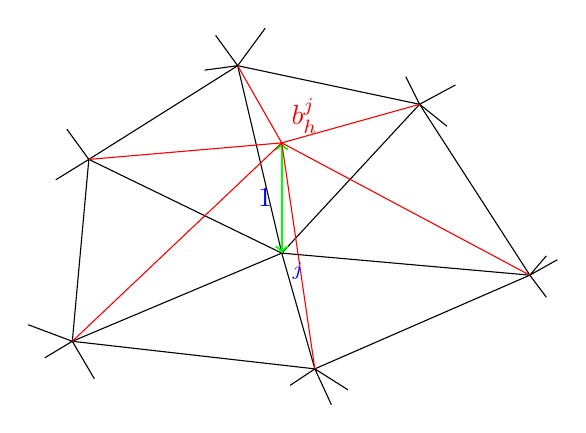
\begin{tikzpicture}[scale=.7]
%            (D)
%		    /   \
%     (E)  /	 \ (C)
%		  |	      |
%     (F) |	      | (B)
%  	       \     /  
%           \   / 
%            (A)

	\coordinate (O) at (0,0); \coordinate (T) at (0,2);
	\coordinate (A) at (0.6,-2.1);
	\coordinate (B) at (4.5,-0.4);
	\coordinate (C) at (2.5,2.7);
	\coordinate (D) at (-0.8,3.4);
	\coordinate (E) at (-3.5,1.7);
	\coordinate (F) at (-3.8,-1.6);
	\draw (A)--(B)--(C)--(D)--(E)--(F)--(A);
	\draw (O)--(A) (O)--(B) (O)--(C) (O)--(D) (O)--(E) (O)--(F);	
	
	\draw (A)-- +(-.45,-.3) 	(A)-- +(.3,-.65)	 (A)-- +(.6,-.38);
	\draw (B)-- +(.3,-.4) 		(B)-- +(.3,.35)	 	 (B)-- +(.5,.28);
	\draw (C)-- +(-.25,.5) 		(C)-- +(.65,.35)	 (C)-- +(.5,-.4);
	\draw (D)-- +(-.6,-.08) 	(D)-- +(-.4,.55)	 (D)-- +(.5,.68);
	\draw (E)-- +(-.6,-.37) 	(E)-- +(-.4,.55);
	\draw (F)-- +(-.8,.3) 		(F)-- +(-.5,-.3)	 (F)-- +(.4,-.68);
	
	\draw[green,thick,<->] (O)--(T);
	\draw[red] (T)--(A) (T)--(B) (T)--(C) (T)--(D) (T)--(E) (T)--(F);
	\node[text=blue,anchor=east] at (0,1) {$1$};
	\node[text=blue,anchor=north] at (0.3,0) {$\bx_j$};
	\node[text=red,anchor=south west] at (0,2) {$b_h^j$}; 
	
\end{tikzpicture}
